\documentclass[10pt]{article}

%----------------------------------------------------------------------------------------
%	Packages and configuration
%----------------------------------------------------------------------------------------

\usepackage[T1]{fontenc}
\usepackage{ucs} % Encoding errors
\usepackage[francais]{babel}
\usepackage{xltxtra} % More XELATEX
\usepackage{graphicx} % Permits to include some pictures
\usepackage{fontspec}
\usepackage{url} % Url links
\usepackage{float} % Adds options to floats like H
\usepackage[ocgcolorlinks]{hyperref}
\usepackage{fancyhdr}
\usepackage{metalogo}
\usepackage[titletoc]{appendix}
\usepackage{pdflscape} % Pour des pages au format paysage
\usepackage{enumitem}  % Pour pouvoir choisir le symbole de itemize : 
                       % \begin{itemize}[label={$\bullet$}]
\usepackage{tabu}
\usepackage{tabularx}
\usepackage{multirow}
\usepackage{lastpage}
\usepackage{multicol}
\usepackage{wrapfig}
\usepackage{longtable}
\usepackage[left=3.5cm,right=3.5cm,top=2cm,bottom=2cm]{geometry} % Change margins
\usepackage[square]{natbib}
\hypersetup{colorlinks=true,allcolors=black}

\setmainfont{Sorts Mill Goudy}
% \setmainfont[BoldFont={Exo},
%   BoldFeatures={Weight=4,Scale=0.9}]{Sorts Mill Goudy}

% \usepackage{sectsty}
% \allsectionsfont{
%   \fontspec[BoldFont={Sorts Mill Goudy}]{Sorts Mill Goudy}}
\pagenumbering{arabic}
\urlstyle{same}
\tabulinesep =1mm
%----------------------------------------------------------------------------------------
%	Header
%----------------------------------------------------------------------------------------

\newcommand{\helv}{%
   \fontsize{9}{11}\selectfont}

   \lhead{\helv \parbox[b]{3.0cm}{ÉTS - Département de génie logiciel et des TI}}
   \chead{\helv \parbox[b]{7cm}{\centering LOG792 - Rapport d'étape - Optimisation des paramètres d’une éolienne en mouvement}}
\rhead{\helv \today \linebreak \thepage}
\lfoot{}
\cfoot{}
\rfoot{}

\setlength{\headwidth}{\textwidth}
\setlength{\headheight}{23pt}

\renewcommand{\headrulewidth}{0.4pt}
%\renewcommand{\footrulewidth}{0.4pt}

%----------------------------------------------------------------------------------------
%	Document
%----------------------------------------------------------------------------------------

\begin{document}

\pagestyle{fancy}

%----------------------------------------------------------------------------------------
%	Page titre
\begin{titlepage}
\thispagestyle{fancy}

\newcommand{\HRule}{\rule{\linewidth}{0.5mm}} % Defines a new command for the horizontal lines, change thickness here

\center % Center everything on the page
 
%----------------------------------------------------------------------------------------
%	HEADING SECTIONS
%----------------------------------------------------------------------------------------

\textsc{\LARGE École de Technologie Supérieure}\\[1.5cm] % Name of your university/college

\vfill

\textsc{\Large Rapport d'étape}\\[0.5cm] % Major heading such as course name
\textsc{\large Projet de fin d'études \\ Département de génie logiciel et des TI}\\[0.5cm] % Minor heading such as course title

%----------------------------------------------------------------------------------------
%	TITLE SECTION


\HRule \\[0.4cm]
{ \huge \bfseries Optimisation des paramètres d’une éolienne en mouvement}\\[0.4cm] % Title of your document
\HRule \\[1.5cm]
 
%----------------------------------------------------------------------------------------
%	AUTHOR SECTION

\begin{minipage}{0.4\textwidth}
\begin{flushleft} \large
\emph{Auteur:}\\
Pierre-Alexandre \textsc{St-Jean}\\
\small{<pa@stjean.me>}
\end{flushleft}
\end{minipage}
~
\begin{minipage}{0.4\textwidth}
\begin{flushright} \large
\emph{Superviseur:} \\
Dr. Christian \textsc{Desrosiers}\\
\small{<christian.desrosiers@etsmtl.ca>}
\end{flushright}
\end{minipage}\\[4cm]

\vfill

%----------------------------------------------------------------------------------------
%	DATE SECTION


{\large \today}\\[3cm] % Date, change the \today to a set date if you want to be precise

%----------------------------------------------------------------------------------------
%	LOGO SECTION

%\includegraphics{Logo}\\[1cm] % Include a department/university logo - this will require the graphicx package

 

\end{titlepage}



%----------------------------------------------------------------------------------------
%	Table des matières
\section*{Table des matières}
% \addcontentsline{toc}{section}{Table des matières}
\renewcommand{\contentsname}{Table des matières}
\makeatletter
\renewcommand{\tableofcontents}{\@starttoc{toc}%
}
\makeatother
\begin{multicols}{2}
\tableofcontents
\end{multicols}
\phantomsection
%\listoffigures
%\addcontentsline{toc}{section}{Table des figures}
%\clearpage

% \vspace*{\fill}
% \begin{center}

\clearpage
%\begin{multicols}{2}
%----------------------------------------------------------------------------------------
%	Abstract
\section*{Résumé}
\addcontentsline{toc}{section}{Résumé}

Le club étudiant Chinook de l'ÉTS afin de continuer son succès en compétition améliore continuellement son véhicule éolien. Un système de contrôle pour l'éolienne tel que celui présent dans les éoliennes statiques doit être mis en place afin d'améliorer la performance du véhicule. Le contrôle de l'angle d'attaque et de la vitesse de rotation de l'éolienne est la façon la plus commune d'ajuster la puissance de sortie d'une éolienne. Afin d'arriver à optimiser le système, l’éolienne du véhicule est d’abord caractérisée expérimentalement puis un système de contrôle de l'angle d'attaque et du ratio de transmission par algorithme génétique est développé, analysé et testé théoriquement et expérimentalement. Le système de contrôle utilisé n'est pas un système conventionnel (PI,PID,etc.) auquel une seule entrée et une seule sortie est considérée, mais plutôt un système dans l'espace d'état dans lequel plusieurs entrées et plusieurs sorties sont considérées.

Résumé des résultats à venir ...


%----------------------------------------------------------------------------------------
%	Intro
\section{Introduction} % (fold)
\label{sec:Introduction}

\subsection{Problématique et contexte} % (fold)
\label{sub:prob_contexte}

Le club étudiant Chinook\footnote{\url{http://chinookets.com}} de l'ÉTS est un regroupement d'étudiants qui analysent, concoivent et construisent un véhicule propulsé par une éolienne [figure \ref{fig:chinookHall}]. Le véhicule participe, chaque année, depuis deux années à une compétition de véhicules du même type et participe à des courses contre la montre. Le véhicule est ensuite évalué selon sa performance en fonction de sa vitesse par rapport à la vitesse du vent.

La compétition vise à ammener les étudiants a développer de nouvelles technologies pour les éoliennes, plus précisément pour des éoliennes de petites dimensions. Afin de rendre la compétition intéressante, elle sont utilisées en tant que moteur d'un véhicule de petite dimension. Un tel véhicule ne serait pas viable mais une telle technologie pourrait facilement être adapté sur d'autre médiums tels que les éoliennes sur des navires ou pour des batiments.

\begin{figure}[H]
  \centering
  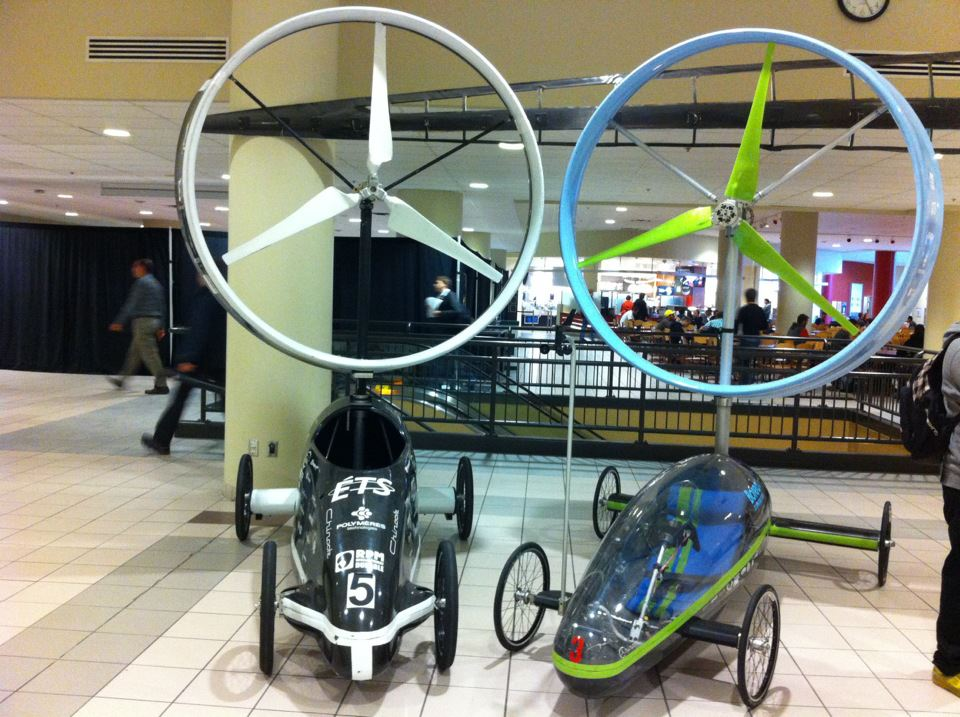
\includegraphics[width=0.5\textwidth]{images/chinook_1_2.jpg}
  \caption[Chinook 1 et 2]{Le Chinook 1 et le Chinook 2 en exposition dans le Hall A de l'ÉTS}
  \label{fig:chinookHall}
\end{figure}

Pour améliorer le véhicule, permettre de à l'équipe de bien performer et rester compétitif l'équipe installe un système électro-mécanique de contrôle de l'angle d'attaque des pâles. La transmission du véhicule sera aussi modifiée afin de pouvoir être asservi électroniquement.

Afin de pouvoir contrôller ces systèmes électroniques, des modèles de contrôle et d'optimisation de la puissance de l'éolienne doivent être créés. Les modèles disponibles sur les éoliennes statique peuvent s'appliquer pour une éolienne en mouvement mais doivent être modifiés afin de prendre en compte plusieurs facteurs.

%--------------------------------------------------------
%--TODO: ------------------------------------------------
... réciter les papers ici
%--------------------------------------------------------
%--------------------------------------------------------

% subsection Problématique et contexte (end)
\subsection{Objectifs} % (fold)
\label{sub:Objectifs}

% subsection Objectifs du projet (end)

% section Introduction (end)


%----------------------------------------------------------------------------------------
%	Methodologie
\section{Méthodologie} % (fold)
\label{sec:Méthodologie}

\subsection{Gestion du projet} % (fold)
\label{sub:Gestion du projet}

% subsection Gestion du projet (end)
\subsection{Analyse du modèle} % (fold)
\label{sub:Analyse du modèle}

% subsection Analyse du modèle (end)
\subsection{Intégration du modèle} % (fold)
\label{sub:Intégration du modèle}

% subsection Intégration du modèle (end)
% section Méthodologie (end)


%----------------------------------------------------------------------------------------
%	Resultats
\section{Résultats} % (fold)
\label{sec:resultats}

\subsection{Sommaire des travaux réalisés} % (fold)
\label{sub:Sommaire des travaux réalisés}

% subsection Sommaire des travaux réalisés (end)
\subsection{Recommandations} % (fold)
\label{subsec:Recommandations}

% subsection Recommandations (end)
% section resultats (end)


%\end{multicols}
%----------------------------------------------------------------------------------------
%	Resultats
\section{Planification} % (fold)
\label{sec:Planification}

L'état d'avancement du projet peut être consulté sur Trello à l'adresse suivante : 
\\
\url{https://trello.com/board/wind-apprentice/518a9dfd2d4ebe4e1a000b36}


\begin{figure}[H]
\label{fig:planif}
\centering
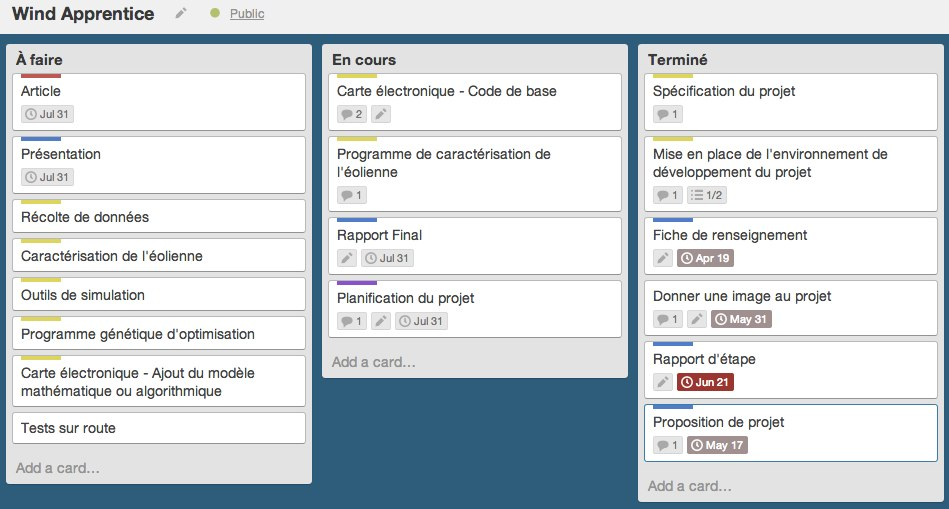
\includegraphics[width=\textwidth]{images/avancement.jpg}
\caption{Planification du projet sur Trello}
\end{figure}

\begin{tabu} to \linewidth {Xlll}
  \textbf{Tâche} & \textbf{Début - Fin} & \textbf{Effort estimé}\\ \hline
  Fiche de renseignement  & 26 Mars 2013 & 1h \\
  Proposition de projet   & 6 Mai 2013 - 12 Mai 2013 & 15h \\
  Rapport Étape           & 12 Mai 2013 - 21 Juin 2013 & 25h\\
  Rapport Final           & 21 Juin 2013 - 31 Juillet 2013 & 30h\\
  Présentation            & 21 Juin 2013 - 31 Juillet 2013 & 5h \\
  Planification du projet & 8 Mai 2013 - 31 Juillet 2013   & 5h\\
  Compétition Racing Aeolus 2013 & 17 Août & \\
  \hline
  Rencontre avec professeur superviseur & (Au besoin) & 3h (1h)\\
  Rencontre avec François Dubé, étudiant de maitrise spécialisé dans le contrôle des éoliennes
  & & 2h \\
  \hline
  Mise en place de l'environnement de développement & 12 Mai - 18 Mai & 5h \\
  Spécification du projet & 12 Mai - 1 Juin & 15h \\
  \hline
  Programme de caractérisation de l'éolienne & 12 Mai - 30 Mai & 15h\\
  Récolte de données                         & Mi-juin & 12h \\
  Caractérisation de l'éolienne              & Mi-juin & 6h\\
  \hline
  Outils de simulation \& de visualisation   & 12 Mai & 30h \\
  Programme génétique d'optimisation         & 1 Juin - 15 Juillet & 30h \\
  \hline
  Carte électronique: implémentation de base    & 10 mars 2013 - 20 Mai 2013 & 30h \\
  Carte électronique: ajout du logiciel d'optimisation & 1 Juillet 2013 - 31 Juillet 2013 & 20h \\
  \hline
  Tests sur route & Mi-Juillet & 3 fois 6h \\
  \hline
\end{tabu}
\subsection{Artéfacts} % (fold)
\label{sub:artefacts}

\begin{longtabu} to \linewidth {X[1,l]X[2,l]}
  \textbf{Artéfact} & \textbf{Description} \\ \hline
  Proposition de projet & Le présent document qui décris sommairement en quoi consistera le projet, ça planification et la façon dont il sera exécuté.\\ \hline
  Rapport d'étape & Document décrivant l'avancement du projet et la façon dont le projet est analyser et conçu \\ \hline
  Rapport final & Document décrivant le projet dans son ensemble.\\ \hline
  Présentation & Préparation et mise en page de la présentation du projet au département de Génie Logiciel et des TI à la fin de la session\\ \hline
  Article & Article scientifique décrivant la méthode utilisée pour caractériser l'éolienne et créer l'algorithme d'optimisation (intégré dans le rapport)\\ \hline
  Spécifications & Documents de spécifications des différents sous-projets que ce projet génère. Sous forme de *readme* dans chaque sous-projet\\ \hline
  Carte électronique: implémentation de base & Implémentation permettant de faire fonctionner tout les composantes de la carte électronique et prêt à accueillir la fonction de calcul. Cet implémentation permet de faire fonctionner les modules de communication soit le XBEE, le module CAN et le module de USB-SERIAL. L'implémentation permettra aussi de faire fonctionner le module de mémoire morte (EEPROM), le module de surveillance électrique et le module d'horloge (realtime clock).\\ \hline
  Carte électronique: Logiciel d'optimisatione & Implémentation du logiciel d'optimisation génétique à l'intérieur de la carte électronique en language C\\ \hline
  Programme de caractérisation de l'éolienne & Programme d'algorithme génétique faisant une opération de Curve-fitting \\ \hline
  Outils de simulation & Outils mathématiques permettant de simuler le fonctionnement de l'éolienne dans des conditions réelles. \\ \hline
  Algorithme génétique d'optimisation & Algorithme permettant d'optimiser les paramètres de l'éolienne selon des conditions quasi réelles d'opération \\ \hline
  Données de banc d'essai & Données récoltés en fixant certains paramètres de l'éolienne. \\ \hline
  Algorithme génétique de caractérisation de l'éolienne & Algorithme permettant de caractérisé la fonction de puissance de l'éolienne en fonction des données récoltés \\ \hline 
  Outils de simulation \& de visualisation & Outils mathématiques et algorithmiques qui permettent de simuler des conditions fictive et de voir les performances de l'éolienne et des algorithmes selon ces conditions\\
  Planification de projet & La planification de projet initiale est produite à l'intérieur de ce document. Elle ensuite continuée sur la plateforme Trello (Voir la section \ref{sec:techoutils}) \\
   Environnement de développement & L'environnement de développement est l'ensemble des outils utilisés lors de ce projet. L'environnement de développement permet de bien intégrer les différents outils entre eux.
\end{longtabu}

% subsection Description des artéfacts (end)
\subsection{Risques} % (fold)
\label{sub:Risques}

\subsubsection{Risques et mitigation de ces risques}

\begin{table}[H]
  \begin{center}
\begin{tabu} to \linewidth {X[1.5,l]|X[3,l]}
  \textbf{Risque} & \textbf{Description} \& \textbf{Mitigation} \\ \hline
  Risque que la préparation du véhicule ne respecte pas les délais & Ce risque peut-être mitigé en ayant un bon suivi de l'avancement et de la construction du véhicule et en offrant de l'aide si nécéssaire. \\ \hline
  Complexité du domaine d'application & Le domaine de l'application des énegies éoliennes et de la mécanique des fluides est un domaine complexe, ce risque peut être mitigé en ayant les bons renseignements en main. Plusieurs ressources sont disponible, soit à l'intérieur du club étudiant Chinook ou auprès des professeurs spécialisés dans ce domaine.\\ \hline
  Manque de données & En s'assurant d'obtenir assez de données lors des sorties de banc d'essai, ce risque est facillement évitable.\\ \hline
  Non fonctionnement de la méthode d'optimisation & Ce risque peut être évité en se renseignant sur l'application et la pertinance de la méthode utilisée. Toutefois, la méthode manuelle de contrôle reste toujours disponible.\\ \hline
  Complexité du projet & Ce risque peut être évité en se documentant correctement sur les méthodes utilisés et en s'assurant de la compréhension de ces méthodes \\
\end{tabu}
  \end{center}
\end{table}

\subsubsection{Impact, probabilité et exposition aux risques}
\begin{table}[H]
  \begin{center}
    \begin{tabu} to \linewidth {X[3.5,l]|X[0.7,l]|X[1,l]|X[1,l]}
      \textbf{Risque}          & \textbf{Impact} & \textbf{Probabilité} & \textbf{Exposition} \\ \hline
      Risque que la préparation du véhicule ne respecte pas les délais & Élevé & Élevé & 0.3734 \\ \hline
      Complexité du domaine d'application & Moyen & Haut   & 0.1698            \\ \hline
      Manque de données                   & Haut  & Faible & 0.0679            \\ \hline
      Non fonctionnement de la méthode d'optimisation & Haut & Faible & 0.0679 \\ \hline
      Complexité du projet                & Moyen & Bas    & 0.0309            \\
    \end{tabu}
  \end{center}
\end{table}


La façon de calculer l'impact des risques et leur probabilités est faite selon la méthode de PÉRIL\footnote{\url{http://msdn.microsoft.com/en-us/magazine/dd315417.aspx}}. Voir les tableaux en [Annexe \ref{annexePERIL}] afin de voir les calculs. 



% subsection Risques (end)
% section Planification (end)


\bibliographystyle{annotate}
%\bibliographystyle{apalike}
%\bibliographystyle{plainnat}
%\bibliographystyle{development}
\bibliography{bibliography}
\addcontentsline{toc}{section}{Références}

%\clearpage

%----------------------------------------------------------------------------------------
%	Annexes
%----------------------------------------------------------------------------------------
\section*{Annexes}
\addcontentsline{toc}{section}{Annexes}
\begin{appendices}



\end{appendices}

\end{document}


